\documentclass[tikz,border=3.14mm]{standalone}
\usepackage{tikz}
\usetikzlibrary{positioning}

\begin{document}

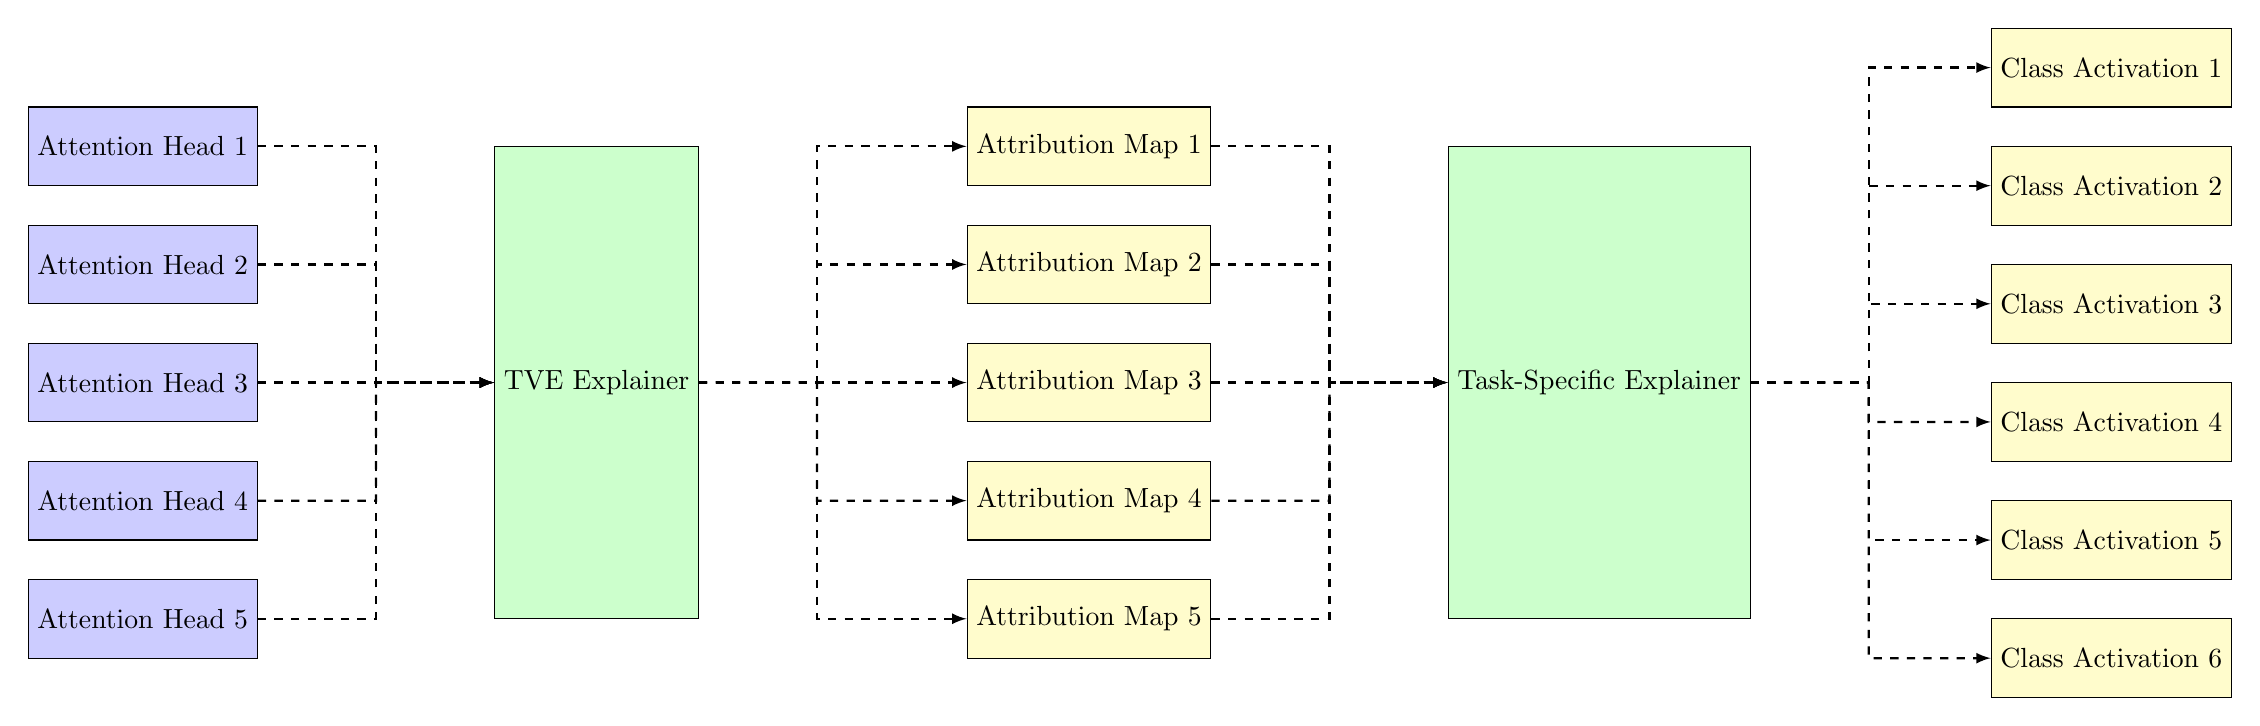
\begin{tikzpicture}[
  head/.style={rectangle, draw=black, fill=blue!20, minimum width=2cm, minimum height=1cm},
  explainer/.style={rectangle, draw=black, fill=green!20, minimum width=2cm, minimum height=6cm, align=center},
  classifier/.style={rectangle, draw=black, fill=red!20, minimum width=2cm, minimum height=1cm},
  attrmap/.style={rectangle, draw=black, fill=yellow!20, minimum width=2cm, minimum height=1cm, align=center},
  arrow/.style={-latex, thick},
  dashedarrow/.style={-latex, thick, dashed}
]

% --- FIRST PART: ATTENTION HEADS TO TVE EXPLAINER ---

% Draw attention heads (backbone layers)
\foreach \i in {1,...,5} {
  \node[head] (h\i) at (0, -\i*1.5) {Attention Head \i};
}

% Draw TVE explainer
\node[explainer, right=3cm of h3] (tve) {TVE Explainer};

% Draw attribution maps at the same height as the attention heads
\foreach \i in {1,...,5} {
  \node[attrmap, right=9cm of h\i] (attr\i) {Attribution Map \i};
}

% Connect all attention heads to TVE explainer (piggyback)
\foreach \i in {1,...,5} {
  \draw[dashedarrow] (h\i.east) -- ++(1.5, 0) -- ++(0, 1.5*\i - 4.5) -- (tve.west);
}

% Connect TVE explainer to attribution maps with rectangular dashed lines
\foreach \i in {1,...,5} {
  \draw[dashedarrow] (tve.east) -- ++(1.5, 0) -- ++(0, -1.5*\i + 4.5) -- (attr\i.west);
}

% --- SECOND PART: ATTRIBUTION MAPS TO TASK-SPECIFIC EXPLAINER ---

% Draw Task-Specific Explainer
\node[explainer, right=3cm of attr3] (task_expl) {Task-Specific Explainer};

% Draw class activations at the same height as the attribution maps
\foreach \i in {1,...,6} {
  \node[attrmap] (class\i) at (25, -1.5*\i +1) {Class Activation \i};
}

% Connect attribution maps to Task-Specific Explainer
\foreach \i in {1,...,5} {
  \draw[dashedarrow] (attr\i.east) -- ++(1.5, 0) -- ++(0, 1.5*\i - 4.5) -- (task_expl.west);
}

% Connect Task-Specific Explainer to class activations
\foreach \i in {1,...,6} {
  \draw[dashedarrow] (task_expl.east) -- ++(1.5, 0) -- ++(0, -1.5*\i + 5.5) -- (class\i.west);
}

\end{tikzpicture}

\end{document}
